\documentclass[sigconf,edbt]{acmart-edbt2021}

\def\BibTeX{{\rm B\kern-.05em{\sc i\kern-.025em b}\kern-.08em
    T\kern-.1667em\lower.7ex\hbox{E}\kern-.125emX}}

\usepackage{booktabs} % For formal tables
\usepackage{tabularx}
\usepackage{tcolorbox}
\newtcbox{\inlinecode}{on line, boxrule=0pt, boxsep=0pt, top=2pt, left=2pt, bottom=2pt, right=2pt, colback=gray!15, colframe=white, fontupper={\ttfamily \footnotesize}}
\usepackage{hyperref}
\hypersetup{
    colorlinks=true,
    linkcolor=blue,
    filecolor=magenta,      
    urlcolor=blue,
}

% Copyright
\setcopyright{rightsretained}


\settopmatter{printacmref=false, printccs=false, printfolios=false}

\pagestyle{empty} % removes running headers


\begin{document}
\title{Data Mining Project's Report}
  

\author{Aurora Maria Tumminello}
\affiliation{%
  \institution{University of Trento}
  \course{1st year, Data Science}
  \city{Trento} 
  \state{Italy} 
}
\email{aurora.tumminello@studenti.unitn.it}

% The default list of authors is too long for headers}
% \renewcommand{\shortauthors}{B. Trovato et al.}
\renewcommand{\shortauthors}{}


\begin{abstract}
This report provides a description of the work related to the data mining project of the academic year 2020/2021. An introduction and motivation will be provided at the start, accompanied by some references to related work from a theoretical perspective. Furthermore, the problem statement and a detailed explanation of the solution proposed will be presented. In conclusion, the report will contain some experimental evaluation.
\end{abstract}

%
% % The code below should be generated by the tool at
% % http://dl.acm.org/ccs.cfm
% % Please copy and paste the code instead of the example below. 
% %
% \begin{CCSXML}
% <ccs2012>
%  <concept>
%   <concept_id>10010520.10010553.10010562</concept_id>
%   <concept_desc>Computer systems organization~Embedded systems</concept_desc>
%   <concept_significance>500</concept_significance>
%  </concept>
%  <concept>
%   <concept_id>10010520.10010575.10010755</concept_id>
%   <concept_desc>Computer systems organization~Redundancy</concept_desc>
%   <concept_significance>300</concept_significance>
%  </concept>
%  <concept>
%   <concept_id>10010520.10010553.10010554</concept_id>
%   <concept_desc>Computer systems organization~Robotics</concept_desc>
%   <concept_significance>100</concept_significance>
%  </concept>
%  <concept>
%   <concept_id>10003033.10003083.10003095</concept_id>
%   <concept_desc>Networks~Network reliability</concept_desc>
%   <concept_significance>100</concept_significance>
%  </concept>
% </ccs2012>  
% \end{CCSXML}
% 
% \ccsdesc[500]{Computer systems organization~Embedded systems}
% \ccsdesc[300]{Computer systems organization~Redundancy}
% \ccsdesc{Computer systems organization~Robotics}
% \ccsdesc[100]{Networks~Network reliability}


% \keywords{ACM proceedings, \LaTeX, text tagging}

%% A "teaser" image appears between the author and affiliation
%% information and the body of the document, and typically spans the
%% page.
\begin{teaserfigure}
  
\includegraphics[width=\textwidth]{sampleteaser.png}
  \caption{Twitter and COVID19}
  \label{fig:teaser}
\end{teaserfigure}

\maketitle

\section{Introduction and Motivation}

The project presented focuses on Twitter data in a specific time period and it aims to identify popular topics contained in tweets. A topic can be considered as a set of terms that regularly can be found together in tweets and that it is popular at a certain time. 

Before talking deeply about the project, some motivations are provided. First of all, we will focus on \textbf{Twitter data}, because they provide a clear overview of events and news in the political, cultural and sociological worldwide sphere. Secondly, \textbf{tweets} are short texts sent at specific times by users all over the world, thus people have to be more directed. In order to do so, they commonly use hashtags, i.e. words preceded by the \inlinecode{\#} character, to spread the word and communicate directly the message with few words. It is interesting to notice that redundancy and ambiguity of natural language are diminished thanks \textbf{hashtags}: they are easy to read, to follow and they communicate directly an idea. Moreover, they become word of mouth and they are frequently used to communicate something that maybe has multiple meanings or way to be told. In addition, Twitter data, contrary to other social networks, are open and downloadable through its API, despite there is a download limit.

The usefulness of this project resides in understanding what is happening in the world, taking into account time and place (when location information is available). Furthermore, to reach this goal, the project aims seeing how words are correlated by looking at how many times they appear together and if they can be considered as a frequent itemset, i.e. as a topic. 

A relevant point to take into consideration is the \textbf{timing} factor, because it bestows a contextual background to topics discovered. If data contextualization was not acknowledged, we would lose all the necessary background for accurate data analysis and interpretation. Therefore, the project presented will look at consistent sets of terms that are frequently used throughout time, i.e. popular topics.

\section{Related Work}
This section aims to provide some useful theoretical works that could help to understand the following steps of this report. 

Before starting to discuss algorithms that could be useful, some text processing clarifications may be necessary. Given the disordered and redundant nature of natural language, data pre-processing is a necessary task in order to evaluate all texts equally and without special characters or distinctions for spaces or case sensitivity. Therefore, taken tweets texts, some steps need to be performed. In particular, we should recur to:

\begin{itemize}
    \item \textbf{RegEx} (regular expression) can be used to identify textual patterns and modify tweets before working on data;
    \item \textbf{stopwords removal}: stopwords are very common words that could alter our analysis with useless topics. For instance, "\textit{and}" could be used in all tweets and all popular words would be in the same set with it, despite it is not so meaningful;
    \item \textbf{stemming}, which is the process of reducing inflexion in words to their root forms. For instance, if we have "\textit{plays}", "\textit{playing}" and "\textit{playful}", the stemmer will reduce all words to "\textit{play}".
\end{itemize}


\section{Problem Statement}
The following function describes which problem we're trying to solve, taking into account the input and the output:

\[ Solution: Date \times Tweet \ Text \rightarrow Topic \times Dates\]

where:
\begin{itemize}
    \item \textit{Date} represents the creation date of the single tweet;
    \item \textit{Tweet Text} stands for the textual corpus of a tweet in a given day;
    \item \textit{Topic} is a frequent itemset, matched with the number of words it contains and the mean ratio in which we can find it in a tweet (i.e. support);
    \item \textit{Dates}, a set of dates in which we can mark a given topic as frequent;
\end{itemize}

\section{Dataset and output description}

The input of the main algorithm presented is a dataset with the date and the cleaned text corpus of tweets, therefore of dimension $N \times 2$, where $N$ represents the number of rows. The \inlinecode{date} column should be a string in the format \inlinecode{YYYY-mm-dd}, while \inlinecode{text} contains tweet body, entire or truncated. If the corpus is truncated, there will be suspension points followed by the link to the referred tweet. The input file should have extension \inlinecode{.csv}. An example of the input file can be found in Table ~\ref{tab:input}.

\begin{table}[h]
\centering
\begin{tabularx}\linewidth{cX}
\toprule
\textbf{date} & \textbf{text}
\\ \midrule
2020-07-25    & {[}'smell', 'scent', 'hand', 'sanit', 'today', 'someon', 'past', 'would', 'think', 'intox'{]}\\
2020-07-25    & {[}'hey', 'yanke', 'yankeespr', 'mlb', 'made', 'sens', 'player', 'pay', 'respect'{]} \\
2020-07-25    & {[}'dian', 'wdunlap', 'realdonaldtrump', 'trump', 'never', 'onc', 'claim', 'covid', 'hoax', 'claim'{]} \\ 
\bottomrule
\end{tabularx}
\caption{Example of input file}
\label{tab:input}
\end{table}

Notice that the solution displayed in this report accepts all dataset that respects those assumptions. Therefore, it can be applied to the \textbf{COVID dataset} used as suggested by the project description, as well as any other Twitter dataset. 

The solution proposed will return as output a set of significant frequent itemsets discovered in the input dataset. The topics contained in the output will be ordered increasingly by the popularity of that topic, i.e. the more that topic is cited in the dataset, the highest position will cover in the results. More in detail, the output will contain: \inlinecode{itemsets}, a list of frequent words recurring together; \inlinecode{n\_items} with the number of words in \inlinecode{itemsets}; \inlinecode{date}, which contains a list of all dates in which the itemset has been frequent; \inlinecode{support}, or the frequent itemset occurrence in proportion to the total number of observations in the dataset. Table ~\ref{tab:output} shows an example of the output described. 

\begin{table}[h]
\centering
\begin{tabularx}\linewidth{lcXc}
\toprule
\textbf{itemsets} & \textbf{n\_items} & \textbf{date}                                 & \textbf{support} \\ \midrule
{[}covid{]}       & 1                 & {[}2020-07-24, 2020-07-25, 2020-07-26, ...{]} & 0.598301         \\
{[}case{]}        & 1                 & {[}2020-07-24, 2020-07-25, 2020-07-26, ...{]} & 0.091421         \\
{[}coronavirus{]} & 1                 & {[}2020-07-24, 2020-07-25, 2020-07-26, ...{]} & 0.077630         \\ \bottomrule
\end{tabularx}
\caption{Output of the project presented}
\label{tab:output}
\end{table}

\section{Dataset}

As depicted in the problem statement, the input should detain only two columns: date and processed text of tweets. Despite that, the original dataset related to COVID19 disposes of the following columns: \inlinecode{user\_name}, \inlinecode{user\_location}, \inlinecode{user\_description}, \inlinecode{user\_created}, \inlinecode{user\_followers}, \inlinecode{user\_friends}, \inlinecode{user\_favourites}, \\ \inlinecode{user\_verified}, \inlinecode{created\_at}, \inlinecode{tweet}, \inlinecode{hashtags}, \inlinecode{source} and \inlinecode{is\_retweet}. As can be noticed, the original dataset contained information about the user who published the tweet, such as username, description, number of followers and location. Related to the latter information (i.e. places where tweets' authors come from) are omitted since there are many missing values. Moreover, location is inserted by users and therefore there is no arbitrary way to indicate, for instance, New York (e.g. \textit{'New York, New York', 'New York, NY, USA', 'Brooklyn, New York', 'New York, LA, Miami, Houston'}). Thus, this project will focus more on the timing instead of the place where topics come from.

In order to obtain the cleaned version of tweets, some computations are necessary, which are contained into \inlinecode{text\_processing.py} file provided:

1. \inlinecode{import\_dataset()}: select only the necessary columns from the original dataset (\inlinecode{created\_at} and \inlinecode{tweet}), changing their names to `date` and `text`. Moreover, only year, month and day are considered, through `date` column conversion to datetime. 

2. \inlinecode{remove\_links()}: removal of internal and final links from tweets (i.e. those words that start with http); 

3. \inlinecode{remove\_symbols()}: this function removes all symbols from tweets (i.e. \textit{\#, @, points, \textbackslash n, \textbackslash r, suspension points} cause by text truncation); 

4. \inlinecode{only\_text()}: the resulting text is divided into many strings, according to the space separator. All non-alphanumerical characters are erased, words are converted to lower case and all remaining symbols or numbers interword are deleted. Notice that numbers were erased only at this step because some words contain numbers in it, such as \textit{covid19} or \textit{covid-19}. In order to disambiguate terms like the previous two (e.g. \textit{covid19, covid-19, covid}), numbers were not considered at all. In the end, empty strings are removed; 

5. \inlinecode{remove\_stopwords()}: taking into consideration only the English vocabulary, all words obtained from previous phases are stemmed to the root. Finally, stopwords are removed, in order not to consider obvious and frequently recurring words, such as \textit{and}.

All these functions are merged inside \inlinecode{text\_processing()}, which is called by \inlinecode{clean\_tweets()} for being computed for each row in the dataset. The new dataframe is then saved in an external file as \inlinecode{input.csv}. Within the project, output files are saved in two formats: \inlinecode{csv}, since it is universally readable; \inlinecode{pickle} format, which allows maintaining columns types without any casting whenever there is the need to import the file. 

In addition to what said about the COVID dataset, it is available at \url{https://www.kaggle.com/gpreda/covid19-tweets} and it refers to the time period from 2020-07-24 to 2020-08-30. The dataset contains 179,108 observations, with 112,733 unique words obtained after text processing. As can be seen in figure ~\ref{fig:termsOccurrence}, where the 20 most recurring terms are shown, nearly all terms occur less than 20K times, except for \textbf{case} and \textbf{covid}, which is the most occurring word in all dataset. Therefore, covid will be probably present in a large number of frequent itemsets.

\begin{figure}[h]
  \centering
  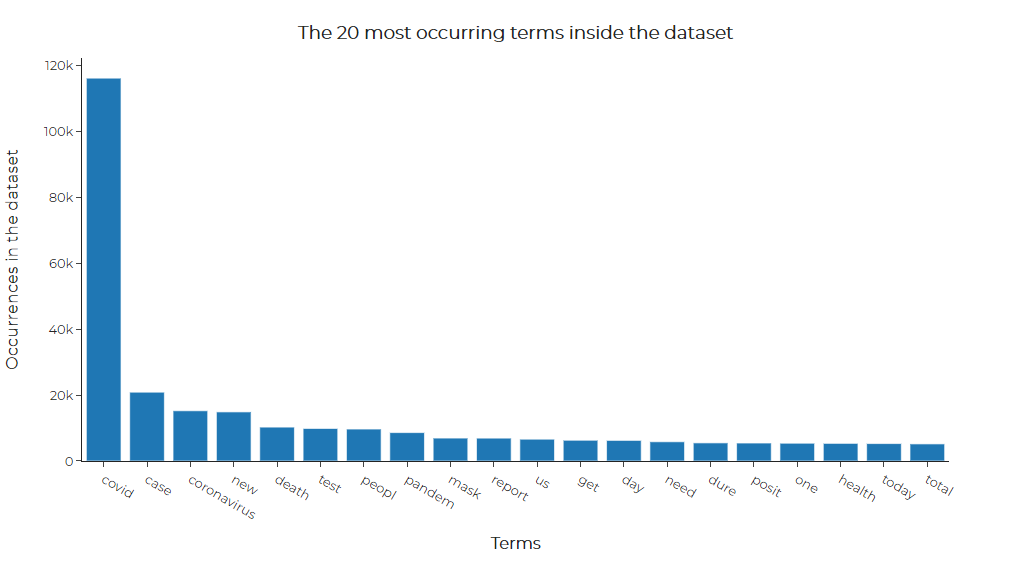
\includegraphics[width=\linewidth]{terms_occurrence.png}
  \caption{The 20 most occurring terms in the COVID19 dataset.}
  \label{fig:termsOccurrence}
\end{figure}

Furthermore, through a deep analysis, it is noticeable that days 2020-07-25 and 2020-08-22 are those in which we can find the highest number of tweets. 

\section{Solution}

\section{Implementation}

\section{Experimental Evaluation}


%%
%% The next two lines define the bibliography style to be used, and
%% the bibliography file.
\bibliographystyle{ACM-Reference-Format}
\bibliography{sample-base}

%%
%% If your work has an appendix, this is the place to put it.
%% Please note that all the content must fit within the page limits, including any appendices.
%\appendix
%
%\section{Research Methods}
% ...

\end{document}
\endinput
